\documentclass[11pt,oneside,a4paper]{article}
\usepackage[margin=1.38in]{geometry}
\usepackage{graphicx}
\usepackage{amsmath}
\usepackage{hyperref}
\usepackage{siunitx}
\usepackage[super]{nth}
\usepackage{pgfplots}
\usepackage{filecontents}
\usepackage{booktabs}
\usepackage{indentfirst}


\graphicspath{ {images/} }

%-------------------------------------------------------------------------------
%	TITLE SECTION
%-------------------------------------------------------------------------------

\newcommand{\horrule}[1]{\rule{\linewidth}{#1}} % Create horizontal rule command with 1 argument of height

\title{
\normalfont \normalsize
\textsc{Sapienza University of Rome} \\ [25pt] % Your university, school and/or department name(s)
\horrule{0.5pt} \\[0.4cm] % Thin top horizontal rule
\LARGE Natural Language Processing \\ % The assignment title
\large Sense Embeddings \\
\horrule{2pt} \\[0.5cm] % Thick bottom horizontal rule
}
\author{Ibis Prevedello} % Your name
\date{\normalsize\today} % Today's date or a custom date

\pgfplotsset{compat=1.15}

\begin{document}

\maketitle




%-------------------------------------------------------------------------------


\section{Introduction}

The goal of this project is to train a Continuous Bag of Words (CBOW) model using Gensim Word2Vec \cite{word2vec} to create a sense embeddings based on the paper 'SENSEMBED: Learning Sense Embeddings for Word and Relational Similarity'\cite{sensembed}.

The dataset used for the training was the EuroSense dataset \cite{eurosense}, which is a multilingual sense-annotated resource in 21 languages, however only the English language was used for this task.

The training was done using a Google Compute Engine instance running a Tesla K80 GPU.

%-------------------------------------------------------------------------------

\section{Network Training}

In order to avoid performing different trainings by hand, a grid search was implemented, where on each execution a different set of variables were tried from a dictionary containing the name of the parameters and a list of values to be tested. At the end of each training the model was evaluated using the The WordSimilarity-353 Test Collection \cite{wordsimilarity}, and if the correlation was better the model was saved.

The total number of trainings performed were 68, divided in three stages, 32 trainings in each of the first two stages and 4 for the last one. The parameters tried were the following: minimum count of each word, window size, embedding size, number of epochs and negative sampling.

%-------------------------------------------------------------------------------

\section{Results}

Tables \ref{tab:first-training} and \ref{tab:second-training} show the correlation value for the first two parameters grid search performed. From the first table it was possible to notice that the negative sampling is really important for the training, obtaining negative values when not considering it, meaning that it causes the vector to point to the opposite direction that it was supposed to.

After noticing the highest correlation of \textbf{0.27} for the first stage, new parameters were chosen and another parameters grid search performed, this time obtaining a big improvement with a correlation of \textbf{0.32}.

For the third stage, it was noticed that the values for minimum count, window and embedding size seemed to be already good, so the embedding size was set to 500 (median value of the highest values of the second stage) and tried increasing the number of epochs and negative sampling. The highest correlation value achieved with only one dataset was \textbf{0.33} and it seems to have no more room to improve only playing with these parameters.

Figure \ref{fig:pca} shows the Principal Component Analysis (PCA), which executes the dimensionality reduction of the 40 words of the BabelNet synset with the highest number of samples. On this image it is possible to notice that some words that are in fact similar tend to stay close in the graph, for example time and year, community and law, country and world, council and debate, and so on.

\begin{table}[]
\centering
\begin{tabular}{@{}rrrrrr@{}}
\toprule
\multicolumn{1}{l}{Min Count} & \multicolumn{1}{l}{Window} & \multicolumn{1}{l}{Embedding} & \multicolumn{1}{l}{Epochs} & \multicolumn{1}{l}{Negative} & \multicolumn{1}{l}{Correlation} \\ \midrule
5 & 3 & 200 & 5 & 0 & -0.138295 \\
5 & 3 & 200 & 5 & 5 & 0.183216 \\
5 & 3 & 200 & 10 & 0 & -0.143903 \\
5 & 3 & 200 & 10 & 5 & 0.243722 \\
5 & 3 & 400 & 5 & 0 & -0.216594 \\
5 & 3 & 400 & 5 & 5 & 0.188902 \\
5 & 3 & 400 & 10 & 0 & -0.216594 \\
5 & 3 & 400 & 10 & 5 & 0.248950 \\
5 & 5 & 200 & 5 & 0 & -0.138295 \\
5 & 5 & 200 & 5 & 5 & 0.244958 \\
5 & 5 & 200 & 10 & 0 & -0.143903 \\
5 & 5 & 200 & 10 & 5 & 0.275019 \\
5 & 5 & 400 & 5 & 0 & -0.216594 \\
5 & 5 & 400 & 5 & 5 & 0.228373 \\
5 & 5 & 400 & 10 & 0 & -0.216594 \\
\textbf{5} & \textbf{5} & \textbf{400} & \textbf{10} & \textbf{5} & \textbf{0.278495} \\
10 & 3 & 200 & 5 & 0 & -0.157774 \\
10 & 3 & 200 & 5 & 5 & 0.174623 \\
10 & 3 & 200 & 10 & 0 & -0.189279 \\
10 & 3 & 200 & 10 & 5 & 0.225277 \\
10 & 3 & 400 & 5 & 0 & -0.230831 \\
10 & 3 & 400 & 5 & 5 & 0.172885 \\
10 & 3 & 400 & 10 & 0 & -0.230831 \\
10 & 3 & 400 & 10 & 5 & 0.229094 \\
10 & 5 & 200 & 5 & 0 & -0.157774 \\
10 & 5 & 200 & 5 & 5 & 0.213183 \\
10 & 5 & 200 & 10 & 0 & -0.189279 \\
10 & 5 & 200 & 10 & 5 & 0.246745 \\
10 & 5 & 400 & 5 & 0 & -0.230831 \\
10 & 5 & 400 & 5 & 5 & 0.211520 \\
10 & 5 & 400 & 10 & 0 & -0.230831 \\
10 & 5 & 400 & 10 & 5 & 0.241750 \\ \bottomrule
\end{tabular}
\caption{Correlation results for the first stage: it was noticed the importance of having negative sampling, 200 not be enough for the embedding size and training for more epochs showing better results.}
\label{tab:first-training}
\end{table}

\begin{table}[]
\centering
\begin{tabular}{@{}rrrrrr@{}}
\toprule
\multicolumn{1}{l}{Min Count} & \multicolumn{1}{l}{Window} & \multicolumn{1}{l}{Embedding} & \multicolumn{1}{l}{Epochs} & \multicolumn{1}{l}{Negative} & \multicolumn{1}{l}{Correlation} \\ \midrule
1 & 5 & 400 & 10 & 5 & 0.124964 \\
1 & 5 & 400 & 10 & 10 & 0.120792 \\
1 & 5 & 400 & 20 & 5 & 0.232549 \\
1 & 5 & 400 & 20 & 10 & 0.276868 \\
1 & 5 & 600 & 10 & 5 & 0.119338 \\
1 & 5 & 600 & 10 & 10 & 0.121477 \\
1 & 5 & 600 & 20 & 5 & 0.229436 \\
1 & 5 & 600 & 20 & 10 & 0.279058 \\
1 & 7 & 400 & 10 & 5 & 0.163271 \\
1 & 7 & 400 & 10 & 10 & 0.118682 \\
1 & 7 & 400 & 20 & 5 & 0.261211 \\
1 & 7 & 400 & 20 & 10 & 0.294953 \\
1 & 7 & 600 & 10 & 5 & 0.154568 \\
1 & 7 & 600 & 10 & 10 & 0.121395 \\
1 & 7 & 600 & 20 & 5 & 0.251919 \\
1 & 7 & 600 & 20 & 10 & 0.294385 \\
5 & 5 & 400 & 10 & 5 & 0.279585 \\
5 & 5 & 400 & 10 & 10 & 0.288543 \\
5 & 5 & 400 & 20 & 5 & 0.306010 \\
\textbf{5} & \textbf{5} & \textbf{400} & \textbf{20} & \textbf{10} & \textbf{0.324633} \\
5 & 5 & 600 & 10 & 5 & 0.275742 \\
5 & 5 & 600 & 10 & 10 & 0.288873 \\
5 & 5 & 600 & 20 & 5 & 0.303674 \\
5 & 5 & 600 & 20 & 10 & 0.323576 \\
5 & 7 & 400 & 10 & 5 & 0.280154 \\
5 & 7 & 400 & 10 & 10 & 0.288799 \\
5 & 7 & 400 & 20 & 5 & 0.309288 \\
5 & 7 & 400 & 20 & 10 & 0.313206 \\
5 & 7 & 600 & 10 & 5 & 0.279864 \\
5 & 7 & 600 & 10 & 10 & 0.288741 \\
5 & 7 & 600 & 20 & 5 & 0.311366 \\
5 & 7 & 600 & 20 & 10 & 0.319772 \\ \bottomrule
\end{tabular}
\caption{Correlation results for the second training: the results were definitely better than the first stage, but still seemed to have some room to improve changing the number of epochs and negative sampling.}
\label{tab:second-training}
\end{table}

\begin{table}[]
\centering
\begin{tabular}{@{}rrrrrr@{}}
\toprule
\multicolumn{1}{l}{Min Count} & \multicolumn{1}{l}{Window} & \multicolumn{1}{l}{Embedding} & \multicolumn{1}{l}{Epochs} & \multicolumn{1}{l}{Negative} & \multicolumn{1}{l}{Correlation} \\ \midrule
5 & 5 & 500 & 20 & 10 & 0.326934 \\
5 & 5 & 500 & 20 & 15 & 0.321759 \\
\textbf{5} & \textbf{5} & \textbf{500} & \textbf{30} & \textbf{10} & \textbf{0.331705} \\
5 & 5 & 500 & 30 & 15 & 0.325737 \\ \bottomrule
\end{tabular}
\caption{Correlation results for the third training: the correlation improved very little, showing a better result for more epochs but nothing very relevant.}
\label{tab:third-training}
\end{table}

\begin{figure}
  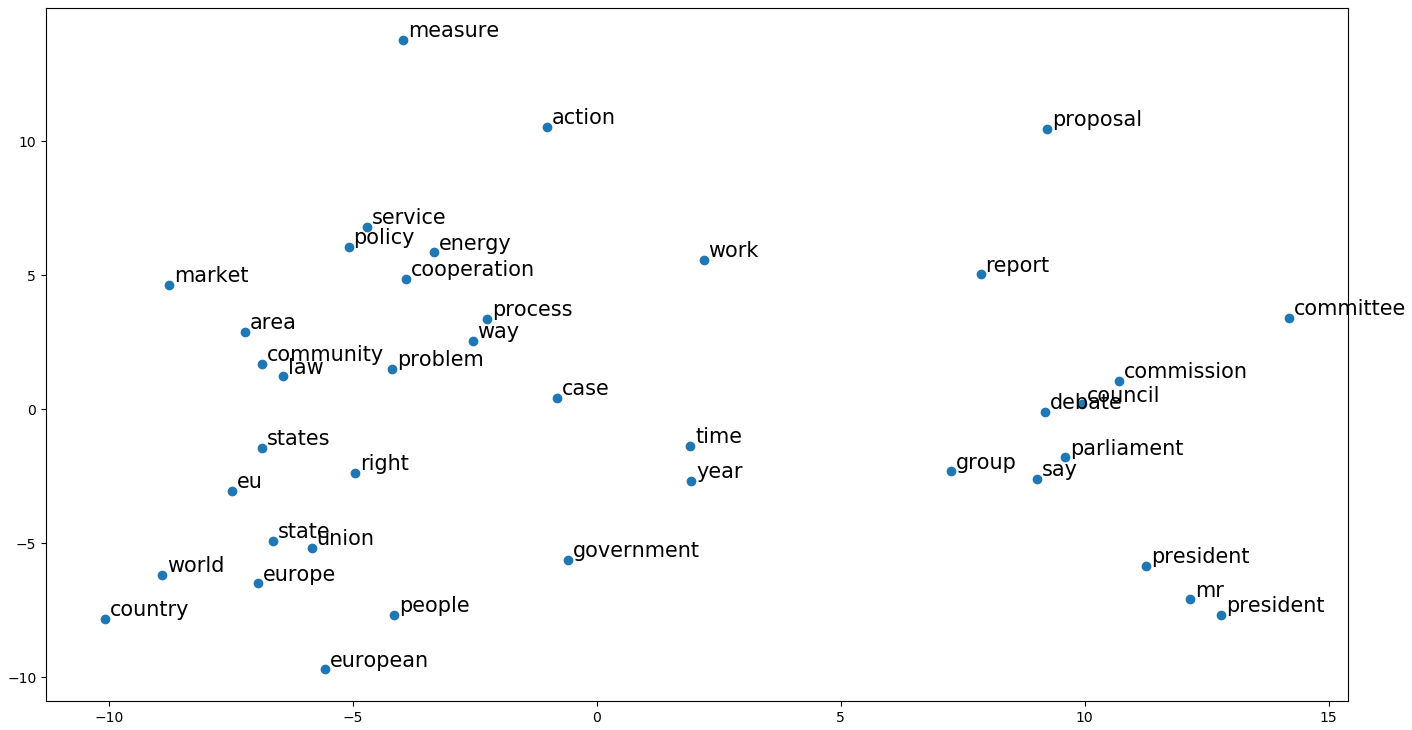
\includegraphics[scale=0.385]{nlp.png}
  \centering
  \caption{Dimensionality reduction of the 40 words of the BabelNet synset with the highest number of samples}
  \label{fig:pca}
\end{figure}

%-------------------------------------------------------------------------------

\section{Conclusion}

The goal of this project was to try different set of parameters using only one dataset and see what was the best correlation that could be achieved and the effects of these parameters in the model.

After all the tests and parameters set tried, the best correlation achieved was \textbf{0.33} using minimum count and window of 5, embedding size of 500, negative sampling of 10 and trained for 30 epochs.

There are a set of other parameters that can be tried for a future project, such as skip-gram instead of CBOW and hierarchical softmax, as well as adding other datasets and training for more epochs.

%-------------------------------------------------------------------------------

\clearpage
\bibliography{bibliography}
\bibliographystyle{ieeetr}

%-------------------------------------------------------------------------------

\end{document}